%%%%%%%%%%%%%%%%%%%%%%%%%%%%%%%%%%%%%%%%%
% Jacobs Landscape Poster
% LaTeX Template
% Version 1.1 (14/06/14)
%
% Created by:
% Computational Physics and Biophysics Group, Jacobs University
% https://teamwork.jacobs-university.de:8443/confluence/display/CoPandBiG/LaTeX+Poster
% 
% Further modified by:
% Nathaniel Johnston (nathaniel@njohnston.ca)
%
% This template has been downloaded from:
% http://www.LaTeXTemplates.com
%
% License:
% CC BY-NC-SA 3.0 (http://creativecommons.org/licenses/by-nc-sa/3.0/)
%
%%%%%%%%%%%%%%%%%%%%%%%%%%%%%%%%%%%%%%%%%

%----------------------------------------------------------------------------------------
%	PACKAGES AND OTHER DOCUMENT CONFIGURATIONS
%----------------------------------------------------------------------------------------

\documentclass[final]{beamer}

\usepackage[scale=1.24]{beamerposter} % Use the beamerposter package for laying out the poster

\usetheme{confposter} % Use the confposter theme supplied with this template

\setbeamercolor{block title}{fg=ngreen,bg=white} % Colors of the block titles
\setbeamercolor{block body}{fg=black,bg=white} % Colors of the body of blocks
\setbeamercolor{block alerted title}{fg=white,bg=dblue!70} % Colors of the highlighted block titles
\setbeamercolor{block alerted body}{fg=black,bg=dblue!10} % Colors of the body of highlighted blocks
% Many more colors are available for use in beamerthemeconfposter.sty

%-----------------------------------------------------------
% Define the column widths and overall poster size
% To set effective sepwid, onecolwid and twocolwid values, first choose how many columns you want and how much separation you want between columns
% In this template, the separation width chosen is 0.024 of the paper width and a 4-column layout
% onecolwid should therefore be (1-(# of columns+1)*sepwid)/# of columns e.g. (1-(4+1)*0.024)/4 = 0.22
% Set twocolwid to be (2*onecolwid)+sepwid = 0.464
% Set threecolwid to be (3*onecolwid)+2*sepwid = 0.708

\newlength{\sepwid}
\newlength{\onecolwid}
\newlength{\twocolwid}
\newlength{\threecolwid}
\setlength{\paperwidth}{48in} % A0 width: 46.8in
\setlength{\paperheight}{36in} % A0 height: 33.1in
\setlength{\sepwid}{0.024\paperwidth} % Separation width (white space) between columns
\setlength{\onecolwid}{0.22\paperwidth} % Width of one column
\setlength{\twocolwid}{0.464\paperwidth} % Width of two columns
\setlength{\threecolwid}{0.708\paperwidth} % Width of three columns
\setlength{\topmargin}{-0.5in} % Reduce the top margin size
%-----------------------------------------------------------

\usepackage{graphicx}  % Required for including images

\usepackage{booktabs} % Top and bottom rules for tables

\usepackage{amsmath}  % for segment functions

%----------------------------------------------------------------------------------------
%	TITLE SECTION 
%----------------------------------------------------------------------------------------

\title{A Numerical Simulation of Volcanic Plume Using SPH Method} % Poster title

\author{Zhixuan Cao, Abani Patra} % Author(s)

\institute{Department of Aerospace and Mechinical Engineering, University at Buffalo, SUNY} % Institution(s)

%----------------------------------------------------------------------------------------

\begin{document}

\addtobeamertemplate{block end}{}{\vspace*{2ex}} % White space under blocks
\addtobeamertemplate{block alerted end}{}{\vspace*{2ex}} % White space under highlighted (alert) blocks

\setlength{\belowcaptionskip}{2ex} % White space under figures
\setlength\belowdisplayshortskip{2ex} % White space under equations

\begin{frame}[t] % The whole poster is enclosed in one beamer frame

\begin{columns}[t] % The whole poster consists of three major columns, the second of which is split into two columns twice - the [t] option aligns each column's content to the top

\begin{column}{\sepwid}\end{column} % Empty spacer column

\begin{column}{\onecolwid} % The first column

%----------------------------------------------------------------------------------------
%	Abstract
%----------------------------------------------------------------------------------------

\begin{alertblock}{Abstract}
\begin{itemize}
\item \textbf{Physics Model} Employ a three dimensional, two phases, transient model based on basic physics laws.\
\item \textbf{Numerical Tools} SPH is suitable for geophysics flow for several reasons: 1) SPH can capture boundary of free boundary flow automatically, 2) treating of multiple phase flow is trival for SPH, 3) adding of new physics requires much less coding effort.\
\item \textbf{Parallel Computing} timeliness and more comprehensive model and finer resolution are conflict demands for prediction capability of numerical simulation, distributed memory parallel computing is adopted.
\item \textbf{Goal} This model is targetting at but not limited to providing source terms for VATDMs (Volcanic Ash Transport and Dispersal Models).
\end{itemize}
\end{alertblock}

%----------------------------------------------------------------------------------------
%	INTRODUCTION
%----------------------------------------------------------------------------------------

%\begin{block}{Introduction}
%The dynamics of explosive eruption clouds has been the central issue of volcanology science for a long time\citep{bullard1962volcanoes, woods1988fluid, valentine1989numerical}. Primary hazards associated with explosive “grey volcanoes” include pyroclastic density currents (flows and surges), the widespread deposition of airfall tephra, and the threats posed by volcanic ash to aviation. In addition, there are also other secondary hazards associated with volcano plume
%Volcanic ash, even in small quantities, poses a significant risk for aircrafts and communities. Most volcanic ash transport and dispersion models (VATDs) take output of a volcano plume model as input. So the accuracy of of plume model is crucial for dispersion simulation. Several volcano plume models adopting mesh-based methods have been developed in the past few decades (e.g. \cite{oberhuber1998volcanic, neri1996numerical, suzuki2005numerical}). SPH method has several advantages over mesh-based methods for modeling volcano plume. 
%We develop a new plume model employing two phases fluid dynamic governing equations and three-dimensional coordinates using SPH method. 
%\end{block}
%------------------------------------------------------------
%Physics Model
%------------------------------------------------------------
\begin{block}{Physics Model \cite{suzuki2005numerical}}
The following assumptions are made:
\begin{itemize}
\item Neglect molecular viscosity.
\item Assume erupted material are well mixed and behave like a single phase fluid all the time.
\item Assume immediate thermodynamics equilibrium and dynamics equilibrium between two phases.
\item Ignore micro-physics process (like phase change of $H_2O$, aggregation, decomposition) and chemical reaction
\end{itemize}.
The governing equations are:
\begin{eqnarray} %%I did not notice that I can add equation like this, useful, haha
\dfrac{\partial \rho}{\partial t} + \nabla \cdot (\rho \textbf{v}) &=& 0 \label{eq:gov-cs-rho} \\
\dfrac{\partial \rho \xi}{\partial t} + \nabla \cdot (\rho \xi \textbf{v}) &=& 0 \label{eq:gov-cs-ks}\\
\dfrac{\partial \rho \textbf{v}}{\partial t} + \nabla \cdot (\rho \textbf{v} \textbf{v} + p\textbf{I}) &=& \rho \textbf{g} \label{eq:gov-cs-v} \\
\dfrac{\partial \rho E}{\partial t} + \nabla \cdot [(\rho E + p )\textbf{v}] &=& \rho \textbf{g} \cdot\textbf{v} \label{eq:gov-cs-e}
\end{eqnarray}
With an additional equation of state to close system of equations.
\begin{equation}
p = (\gamma_m - 1)\rho e \label{eq:EOS}
\end{equation}

\end{block}
\end{column} % End of the first column
%-----------------------------------------------------------------------------------
\begin{column}{\sepwid}\end{column} % Empty spacer
%-----------------------------------------------------------------------------------

%----------------------------------------------------------------------------------
\begin{column}{\onecolwid}\vspace{-.6in} 
%----------------------------------------------------------------------------------------
%	SPH Methods
%----------------------------------------------------------------------------------------
%\begin{block}{SPH Methods}
%SPH method discretize the domain with a set of particles or discretization points and the position of each particle is updated at every time step. Approximation of all field variables (velocity, density and pressure, ect.) is obtained by interpolation based on discretization points. Using a kernel function that provides the weighted estimation of the field variables in the neighborhood of a discrete point (particle). The integral equations are evaluated as sums over neighbor particles. Thus, physical properties (density, velocity, internal energy, ect.) associated to the particle are updated based on its neighbors.
%\end{block}

%--------------------------------------------------------------------------------------
\begin{block}{Shocktube Problems}
\begin{figure}
\centering
{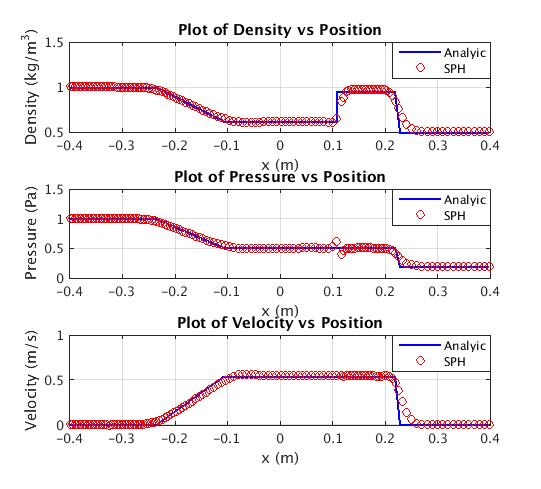
\includegraphics[height= 0.650\linewidth]{shocktube}}
\caption{Solving of a 1D benchmark problem (shock tube) with SPH method, results are consistent with analytic solution}
\label{fig:effect_of_turbulence}
\end{figure}
\end{block}
%----------------------------------------------------------------------------------------

%----------------------------------------------------------------------------------------
%	METHODS
%----------------------------------------------------------------------------------------

\begin{block}{ $SPH-\varepsilon$ Turbulence Model \cite{monaghan2011turbulence}}
Using the ideas associated with the Lagrangian averaged Navier Stokes equations(LANS), a smoothed velocity $\widehat{\textbf{v}}$ 
defined in terms of the unsmoothed velocity $\textbf{v}$ by:
\begin{equation}
\widehat{\textbf{v}}(\textbf{r})=\int \textbf{v}(\textbf{r} \prime)G(\vert \textbf{r} \prime - \textbf{r} \vert, l) d\textbf{r} \prime
\end{equation}
the discretized momentum equation with $SPH-\varepsilon$ turbulence model in our simulation will be:
\begin{equation}
\label{eq:SPH-mom-epsilon-turb}
\dfrac{d \textbf{v}_a}{dt} = -\sum_b [m_b (\dfrac{p_b}{\rho_b^2} + \dfrac{p_a}{\rho_a^2}) \bigtriangledown_aw_{a b}(h_a)] + R_t
\end{equation}
The stresses induced by the smoothing:
\begin{equation}
R_t=\sum_b m_b \dfrac{\varepsilon}{2} \dfrac{\textbf{v}_{ab} \cdot \textbf{v}_{ab}}{\rho_b} \bigtriangledown_aG_{ab}(l_a)
\end{equation}
 
\begin{figure}
\centering
{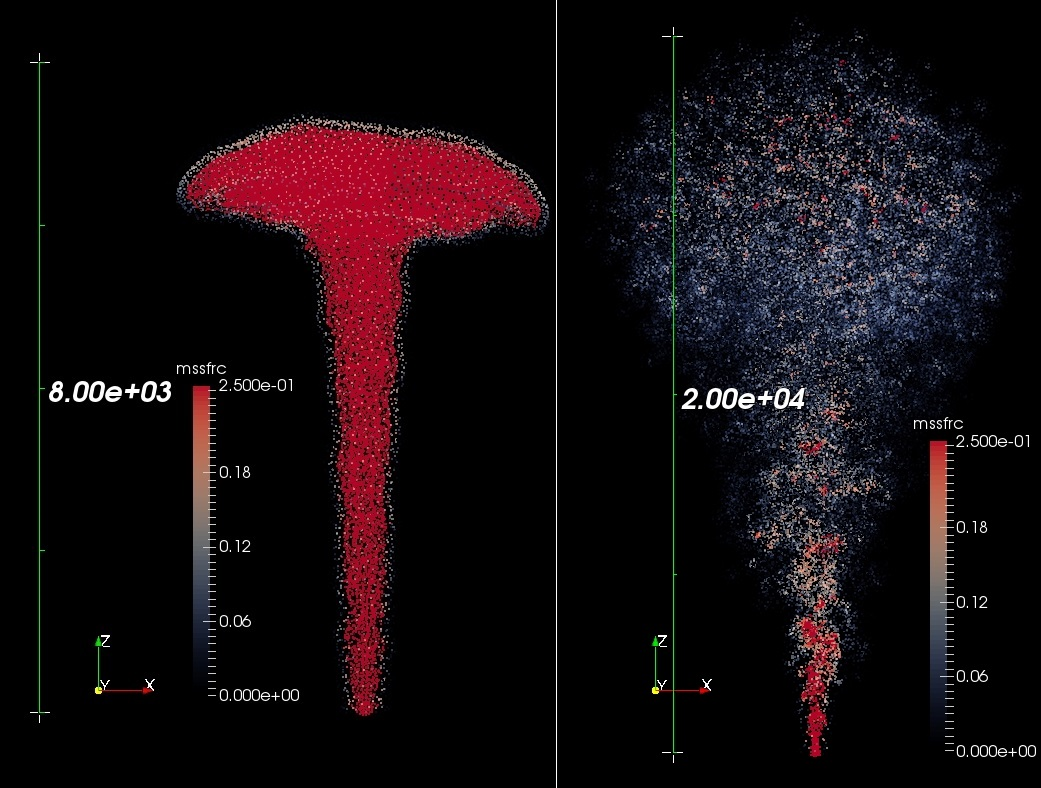
\includegraphics[scale=0.85]{effect_of_turb_model}}
\caption{Simulation results at t=200. When turbulence model is not included (left figure), the entrainment of air is obviously too less that plume will stop raising up after its initial momentum exhuasted.}
\label{fig:effect_of_turbulence}
\end{figure}

\end{block}
%----------------------------------------------------------------------------------------

\end{column} % End of column 2.2

%----------------------------------------------------------------------------------

\begin{column}{\sepwid}\end{column} % Empty spacercolumn

\begin{column}{\twocolwid} % Begin a column which is two columns wide (column 2)

\begin{columns}[t,totalwidth=\twocolwid] % Split up the two columns wide column

\begin{column}{\onecolwid}\vspace{-1.4in} % The first column within column 2 (column 2.1)

%----------------------------------------------------------------------------------------
%	MATERIALS
%----------------------------------------------------------------------------------------
\begin{block}{Simulation of JPUE}

\begin{figure}
\centering
{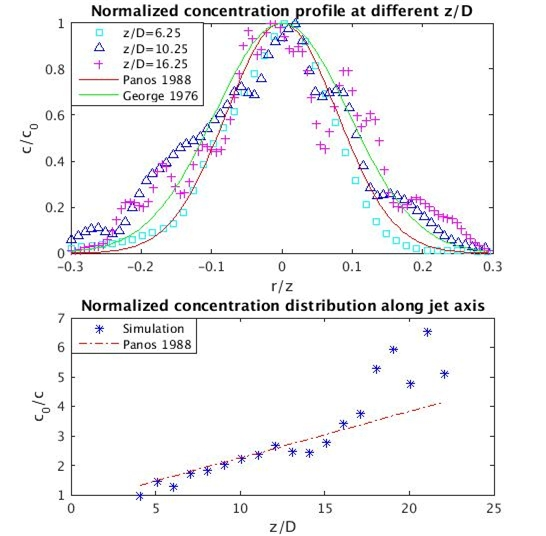
\includegraphics[height= 0.690\linewidth]{jpue_conc}}
\caption{Jet or plume which is ejected from a nozzle into a uniform environment(JPUE) can be viewed as a simplified volcanic plume. Simulation results of JPUE is compared with experimental resutls \cite{papanicolaou1988investigations, george1977turbulence} for verification purpose. Concetration distribution across the cross-section is fit into a Gaussion profile (solid line) even though there is no priori reason. D is the diameter of vent, $c_0$ is concetration at the vent.}
\end{figure}

\end{block}
%----------------------------------------------------------------------------------------

\end{column} % End of column 2.1

\begin{column}{\onecolwid}\vspace{-1.4in} 
%----------------------------------------------------------------------------------------
%	METHODS
%----------------------------------------------------------------------------------------
\begin{alertblock}{References}

%\nocite{*} % Insert publications even if they are not cited in the poster
\small{\bibliographystyle{unsrt}
\bibliography{Reference}}

\end{alertblock}

%-----------------------------------------------------------------------------
% contact information
%---------------------------------------------------------------------------------
%\setbeamercolor{block alerted title}{fg=black,bg=norange} % Change the alert block title colors
%\setbeamercolor{block alerted body}{fg=black,bg=white} % Change the alert block body colors

%\begin{alertblock}{Contact Information}

%\begin{itemize}
%\item Email: \href{mailto:zhixuanc@buffalo.edu}{ abani@buffalo.edu}
%\item Phone: +1 (716) 319 0543
%\end{itemize}

%\end{alertblock}

%----------------------------------------------------------------------------------------

\end{column} %

\end{columns} \vspace{-1.0in}
%----------------------------------------------------------------------------------------
%	IMPORTANT RESULT
%----------------------------------------------------------------------------------------

\begin{block}{Simulation of Volcano Plume}

\begin{figure}
\centering
{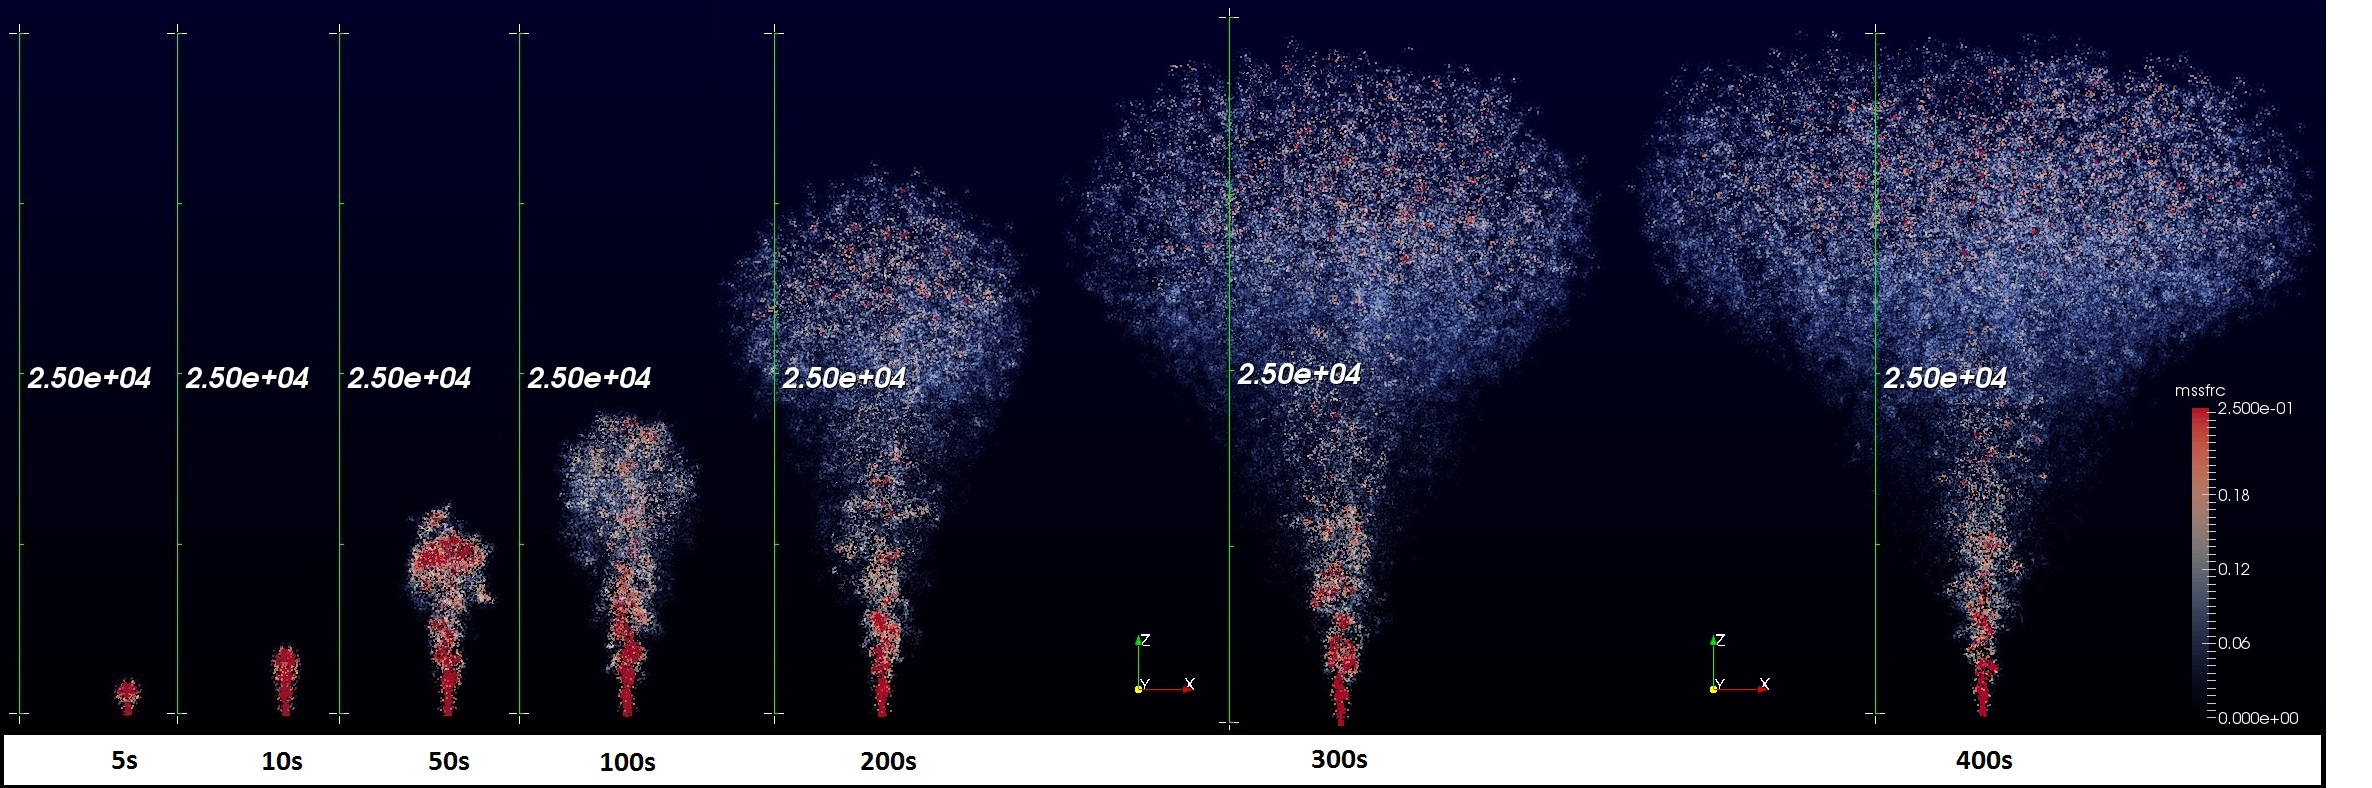
\includegraphics[scale=0.90]{plume_grow_up}}
\caption{Evolution of plume with time. After around 300 seconds, the plume reaches its top height and start expanding}
\end{figure}

\end{block}\vspace{-1.8in}
%----------------------------------------------------------------------------------------

\begin{columns}[t,totalwidth=\twocolwid] \vspace{-1.5in}% Split up the two columns wide column again

\begin{column}{\onecolwid} % The first column within column 2 (column 2.1)

%----------------------------------------------------------------------------------------
%	MATHEMATICAL SECTION
%----------------------------------------------------------------------------------------

\begin{table}
\centering
\caption{Input Parameters for Simulation}
%\caption{Input parameter}\\
\begin{tabular}{|l|l|l|l|l|}
\toprule
\midrule
Radius& Speed& Temperature& Water\%& Mass Flux \\
\hline
140m& 150m/s& 1000K& 0.05& 39810717kg/s\\
\bottomrule
\end{tabular}
%\caption{Table caption}
\end{table}
Atmosphere is determined according to:

\begin{displaymath}
   T_a(z) = \left\{
     \begin{array}{l l}
       T_{a0} - \mu_1 z & \ \ 0\leq z \textless H_1\\
       T_{a0} - \mu_1 H1 & \ \  H_1\leq z \textless H_2 \\
       T_{a0} - \mu_1 H1 + \mu_2 (z-H2) & \ \  z \textgreater H_2
     \end{array}
   \right.
\end{displaymath} 

%----------------------------------------------------------------------------------------

\end{column} \vspace{-1.8in}% End of column 2.1


\begin{column}{\onecolwid} % The second column within column 2 (column 2.2)

%----------------------------------------------------------------------------------------
%	RESULTS
%----------------------------------------------------------------------------------------

\begin{figure}
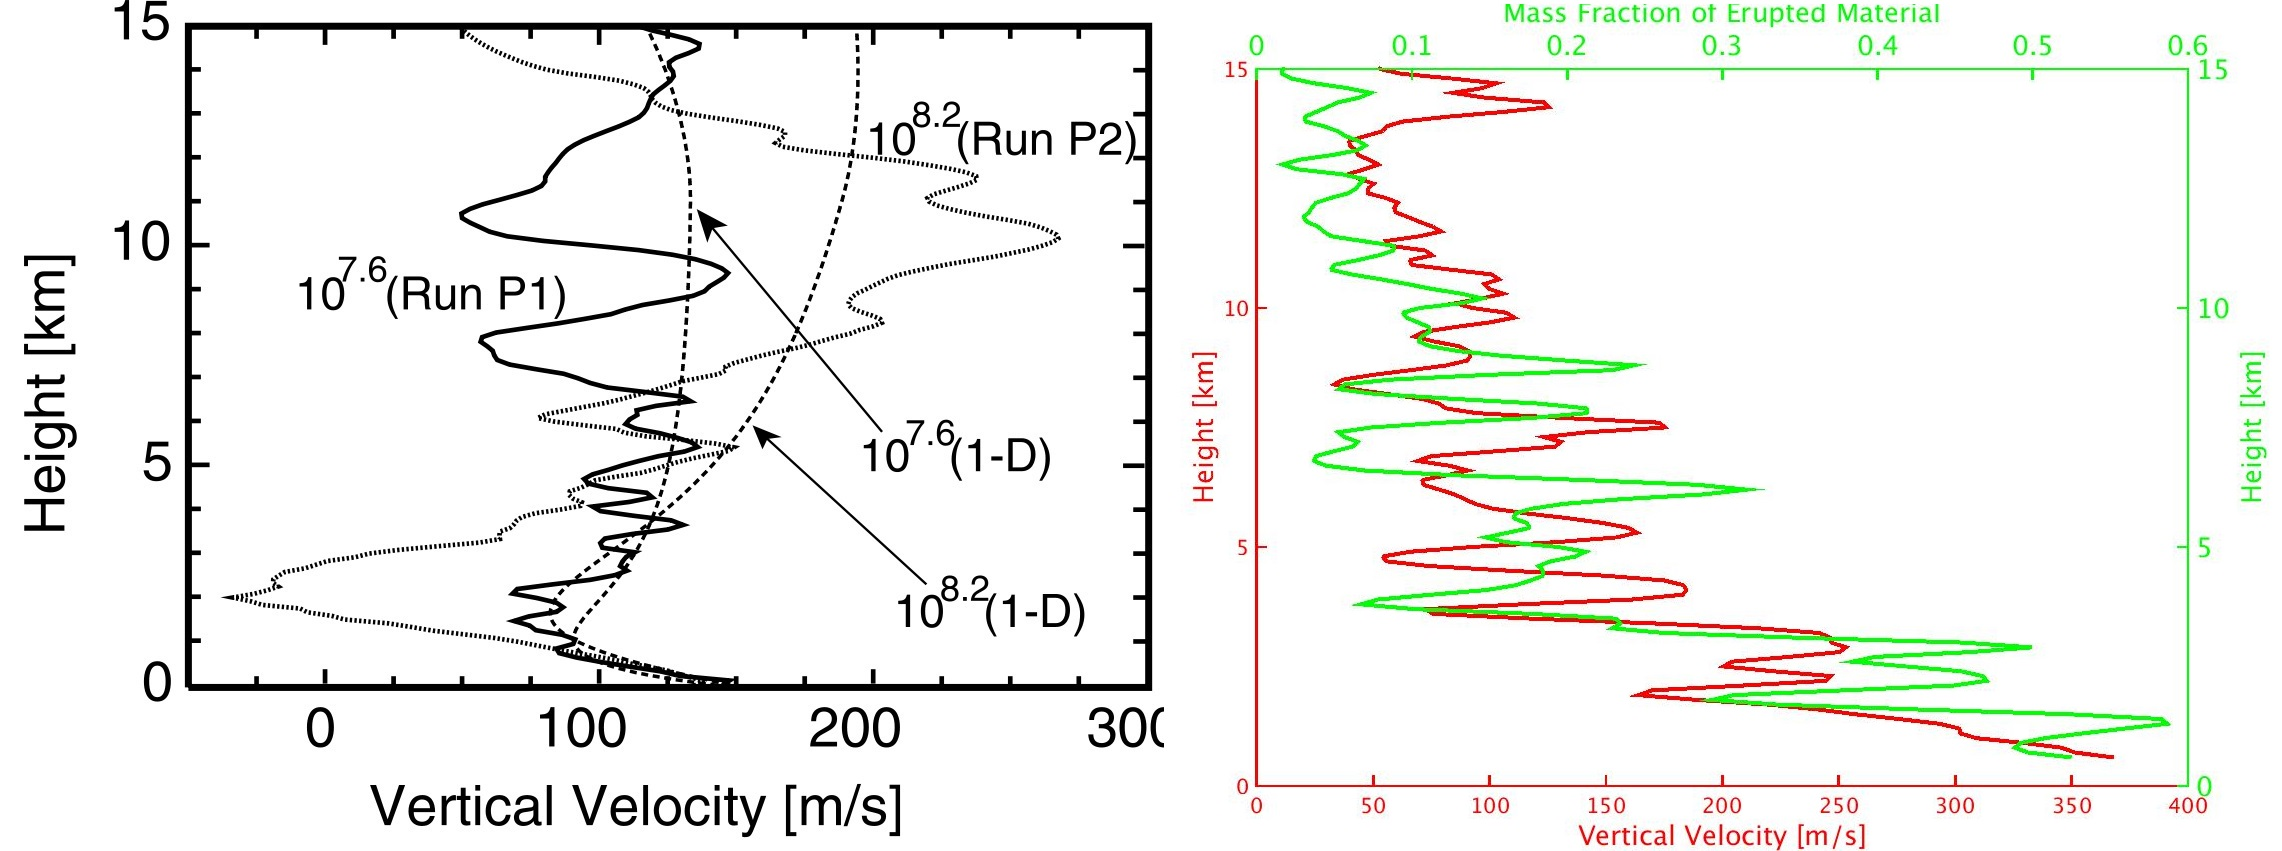
\includegraphics[height= 0.40\linewidth]{Velocity_at_cent}
\caption{Distribution of vertical velocity and mass fraction along central axis of the plume. Input parameters and atmosphere are the same as "Run P1" of left figure\cite{suzuki2005numerical}.}
\end{figure}

%----------------------------------------------------------------------------------------

\end{column} % End of column 2.2

\end{columns} % End of the split of column 2

\end{column} % End of the second column

\begin{column}{\sepwid}\end{column} % Empty spacer column

\begin{column}{\onecolwid} % The third column

%----------------------------------------------------------------------------------------
%	ACKNOWLEDGEMENTS
%----------------------------------------------------------------------------------------

%\setbeamercolor{block title}{fg=red,bg=white} % Change the block title color

%\begin{block}{Acknowledgements}

%\footnotesize{\rmfamily{Nam mollis tristique neque eu luctus. Suspendisse rutrum congue nisi sed convallis. Aenean id neque dolor. Pellentesque habitant morbi tristique senectus et netus et malesuada fames ac turpis egestas.}} \\

%\end{block}

%----------------------------------------------------------------------
%  LOGO
%----------------------------------------------------------------------
%\begin{center}
%\begin{tabular}{ccc}
%
\includegraphics[width=0.2\linewidth]{logo} & \hfill & 
\includegraphics[width=0.2\linewidth]{logo}
%\end{tabular}
%\end{center}

\end{column} % End of the third column

\end{columns} % End of all the columns in the poster

\end{frame} % End of the enclosing frame

\end{document}
